%%%%%%%%%%%%%%%%%%%%%%%%%%%%%%%%%%%%%%%%%%%%%%%%%%%%%%%%%%%%%%%%%%%%%%%%%%%%%%%%
%2345678901234567890123456789012345678901234567890123456789012345678901234567890
%        1         2         3         4         5         6         7         8

\documentclass[letterpaper, 10 pt, conference]{ieeeconf}  % Comment this line out
                                                          % if you need a4paper
%\documentclass[a4paper, 10pt, conference]{ieeeconf}      % Use this line for a4
                                                          % paper

\IEEEoverridecommandlockouts                              % This command is only
                                                          % needed if you want to
                                                          % use the \thanks command
\overrideIEEEmargins
% See the \addtolength command later in the file to balance the column lengths
% on the last page of the document

\usepackage{listings}
\usepackage{biblatex}
\bibliography{paper}
\usepackage{float}
\usepackage{amsmath}
\usepackage{graphicx}
% The following packages can be found on http:\\www.ctan.org
%\usepackage{graphics} % for pdf, bitmapped graphics files
%\usepackage{epsfig} % for postscript graphics files
%\usepackage{mathptmx} % assumes new font selection scheme installed
%\usepackage{times} % assumes new font selection scheme installed
%\usepackage{amsmath} % assumes amsmath package installed
%\usepackage{amssymb}  % assumes amsmath package installed
\lstset{
%  basicstyle=\ttfamily,
  columns=fullflexible,
  frame=single,
  breaklines=true,
  basicstyle=\small
}

\title{\LARGE \bf
Object Detection-Based Behaviour using YOLO on Thymio
}

%\author{ \parbox{3 in}{\centering Huibert Kwakernaak*
%         \thanks{*Use the $\backslash$thanks command to put information here}\\
%         Faculty of Electrical Engineering, Mathematics and Computer Science\\
%         University of Twente\\
%         7500 AE Enschede, The Netherlands\\
%         {\tt\small h.kwakernaak@autsubmit.com}}
%         \hspace*{ 0.5 in}
%         \parbox{3 in}{ \centering Pradeep Misra**
%         \thanks{**The footnote marks may be inserted manually}\\
%        Department of Electrical Engineering \\
%         Wright State University\\
%         Dayton, OH 45435, USA\\
%         {\tt\small pmisra@cs.wright.edu}}
%}

\author{Francesco Saverio Zuppichini$^{1}$ and Alessia Ruggeri$^{2}$}% <-this % stops a space


\begin{document}



\maketitle
\thispagestyle{empty}
\pagestyle{empty}


%%%%%%%%%%%%%%%%%%%%%%%%%%%%%%%%%%%%%%%%%%%%%%%%%%%%%%%%%%%%%%%%%%%%%%%%%%%%%%%%
\begin{abstract}
The ability to classify objects in both space and domain is encoded in an enormous variety of species on the planet. Recently, deep learning approaches have been developed to make machines able to mimic the same task with interesting results. With this paper, we propose a minimal architecture to archive the same goal using a two wheels robots, the Thymio, with a mounted frontal camera in order to make it act based on the objects detected in the surrounding. 
\end{abstract}

\section{Introduction}

Finding objects in space by identifying their identity and their coordinates is a basic task that almost each animal is able to accomplish. The ability to solve this problem is extremely important in robotics, where a machine needs to act accordingly based on its surrounding. With our architecture, only the raw data from the camera are used as input to an Object Detection model and the decision are based directly on the prediction, without the need of any other sensor.

Specifically, our robot will wait for an user-specified class, e.g. \emph{dog}, and, when found, it moves towards the object by keeping it in the middle of its view. We also implemented a PID based algorithm to avoid obstacles and properly stop in front of founded item.

The paper is structured as follows: we will first describe the architecture by showing each individual part of the topology and how they interact; then, we will discuss the challenges during the development process and finally we will show the results.

\section{Architecture overview}
We used ROS\cite{ROS} as operating system to develop and deploy our code on the Thymio. Our architecture is composed by:
\begin{enumerate}
	\item A robot with a mounted camera and an on-board computer
	\item A web server running the Object Detection model
	\item A ROS node running on a local machine that moves the robot
\end{enumerate}
As a robot, we used the \emph{MightyThymio} \cite{guzzi2018eaai}, which is a robot developed on top of the Thymio, a small mass-produced mobile robot usually used in primary and secondary education. The MightyThymio has a powerful Odroid C1 on board, a 1GB quad-core ARM Linux machine, with a HD camera mounted on top. The authors also implemented a ROS node to communicate with it and open-sourced the code.

\subsection*{MightyThymio}

In our project, the MightyThymio has the same configuration proposed in \cite{guzzi2018eaai}. Briefly, the on-board computer expose the Thymios sensors through ROS. Thus, another ROS node can publish and subscribe in order to communicate with its sensors. For example, we can subscribe to the \emph{camera sensors} to get information from the proximity sensors to avoid hitting obstacles. Also, we can simply subscribe to the camera's topic to get both compressed and uncompressed images. 

\begin{figure}[H]
\centering
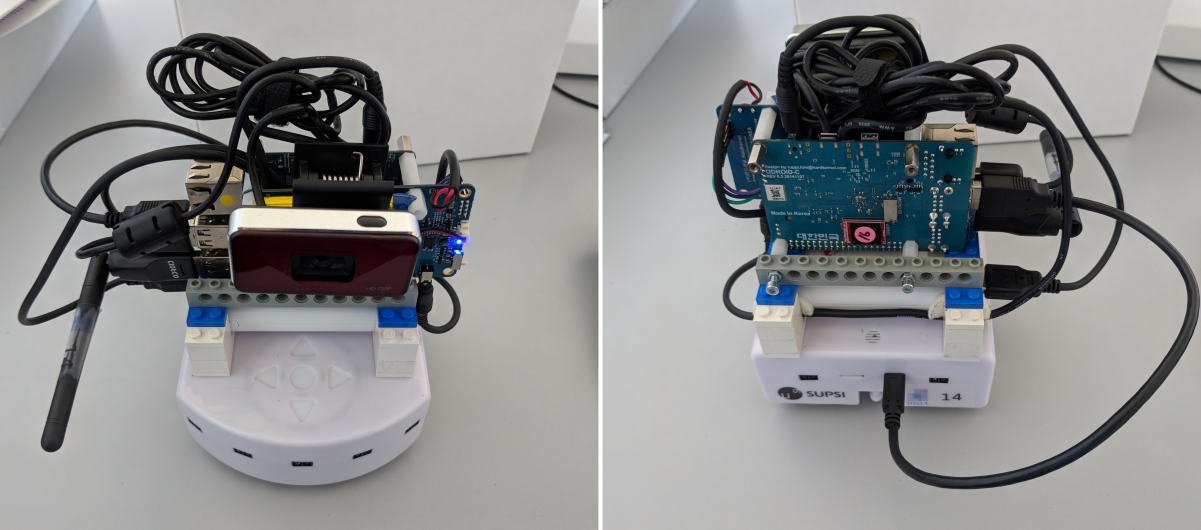
\includegraphics[width=\linewidth]{assembled_myt}	
\caption{The MightyThymio}
\end{figure}
%Subscribe thyme event of camera, from whom compressed images, encoded in strings, then we send to the server, the server decode the compressed images and send prediction. After prediction, if class is target, for example person, the server send the person and bounding box. If the timeo see the person, it moves verso the person keeping her in the centre. So if the person moves, the timeo moves to keep the bounding box in the centre of the camera. So using only the image we can tell timeo to follow a target, without knowing the position of target or of thimeo.
%The rod node is a module that can be put where you want.

\subsection*{Local ROS node}
We created a new ROS node to communicate with the running node on the MightyThymio in order to make it act accordingly with a specified behaviour based on the object detected by the model. The user specifies a set of target classes, for example \emph{dog} and \emph{cat}. Then our node, after having subscribed to the camera topic of the MightyThymio, sends the fetched image to the model trough an HTTP request and gets the bounding boxes for the detected classes. If there is no target prediction, the robot enters in \texttt{exploration} mode and starts spinning around. When one or more of the target classes are found, then our robot will start going forward while keeping the bounding box of the target in the centre of the camera in order to follow it. If we detect more classes, then the closest, which is represented by the biggest bounding box area, will be followed. In addiction, we have an obstacle-avoiding algorithm in order to properly stop the Thymio before it hits the target.

\subsection*{Object Detection REST-API Web Server}
We used pre-trained YOLO\cite{DBLP:conf/cvpr/RedmonDGF16}, the state-of-the-art real-time object detection model, to predict the bounding boxes for each class. The model was trained on the COCO(Common Object in Context)\cite{COCO} Dataset, that contains 80 classes. 

On top of that, we built a REST-API Web Server using Python3 and Flask, a micro-framework to create Web Servers, to make the model accessible from the Web. We decided to decouple the logic behind the robot behaviour and the model in order to make our architecture more scalable. For instance, if needed, we can deploy our model in the cloud while keeping the running ROS code intact. 

We following endpoints are available:
\begin{lstlisting}
GET /model
POST /prediction  --image --size --compress
\end{lstlisting}
Each of them returns a JSON serialised response. The \texttt{/model} endpoint is used to get informations about the model on the server. These informations are the classes and the colour associated to each one of them. It follows a snapshot of the response:
\begin{lstlisting}
{
    "classes": [ "person", "bicycle", "car", "motorbike", "aeroplane", ... ]
    "colors": [[255, 38, 0], [0, 63, 255], ... ]   
 }
\end{lstlisting}
The client can get a prediction by sending and image to \texttt{/prediction}. Also, it can specify whatever the  image is compressed or no and if the server should resize it before feed it to the model. In our case, we send a compressed image directly taken from the MightyThymio after subscribed to the \texttt{/camera/compressed} topic and we define the resize size to (190,190). The small size is due low computational power since we had no access to a GPU. The response looks like:
\begin{lstlisting}
{'res': [{'boxes': [96.21580505371094,
                    219.6134033203125,
                    437.66387939453125,
                    594.16748046875],
          'class': 'bicycle',
          'class_idx': 1,
          'score': 0.48406994342803955}, ...
         ]
 'time': 0.174407958984375}
\end{lstlisting}
For each detected class we return the bounding boxes, the \emph{boxes} key of the json, the class name, its index and the score, the confidence of the model. Each box is composed by the top, left, bottom and right coordinate of the bounding box with respect to the left of the image and the top. In the above example, the bicyle's bounding starts $96$ pixels from the left and $219$ from the top.
\section{}

\subsection{YOLO: Real-Time Object Detection}

YOLO \cite{DBLP:conf/cvpr/RedmonDGF16} is a trained model for real-time object detection. While prior work on object detection repurposes classifiers to perform detection, YOLO handle the object detection as a regression problem to spatially separated bounding boxes and associated class probabilities. YOLO avoids resorting to complex pipelines that are slow and hard to optimize; instead, it uses a single convolutional neural network that simultaneously predicts multiple bounding boxes and class probabilities for those boxes. Using YOLO, You Only Look Once at an image to predict what objects are present and where they are.

YOLO neural network uses features from the entire image to predict each bounding box simultaneously across all classes. The convolutional neural network contains 24 convolutional layers, that extract features from the image, followed by 2 fully connected layers, whose aim is to predict the output probabilities and coordinates. The system divides the input image into an $S \times S$ grid; if the centre of an object falls into a grid cell, that grid cell is responsible for detecting that object. Each grid cell predicts $B$ bounding boxes and confidence scores for those boxes. These confidence scores reflect how confident the model is that the box contains an object and also how accurate it thinks the box is that it predicts. There is also a fast version of YOLO, designed with a neural network with fewer convolutional layers and fewer filters in those layers.

YOLO is extremely fast, it reason globally about the image when making predictions, it learns generalizable representations of objects and it is open source. YOLO still lags behind other detection systems in accuracy; while it can quickly identify object in images, it struggles to precisely localize some objects, especially small ones. However, it is still the state-of-the-art model for object detection in real-time.

For our project, we used the third version of YOLO, or YOLOv3 \cite{Yolo3}, which has been improved by making it a little bigger than before, but more accurate.

\section{Implementation}
We design our ROS node to find object and follow them until it is close enough. In addition, we also implemented a PID based algorithm to avoid obstacle and to stop before crash into the target object. From an high level view, the robot can be represented as a three-state machine.
\begin{figure}[H]
\centering
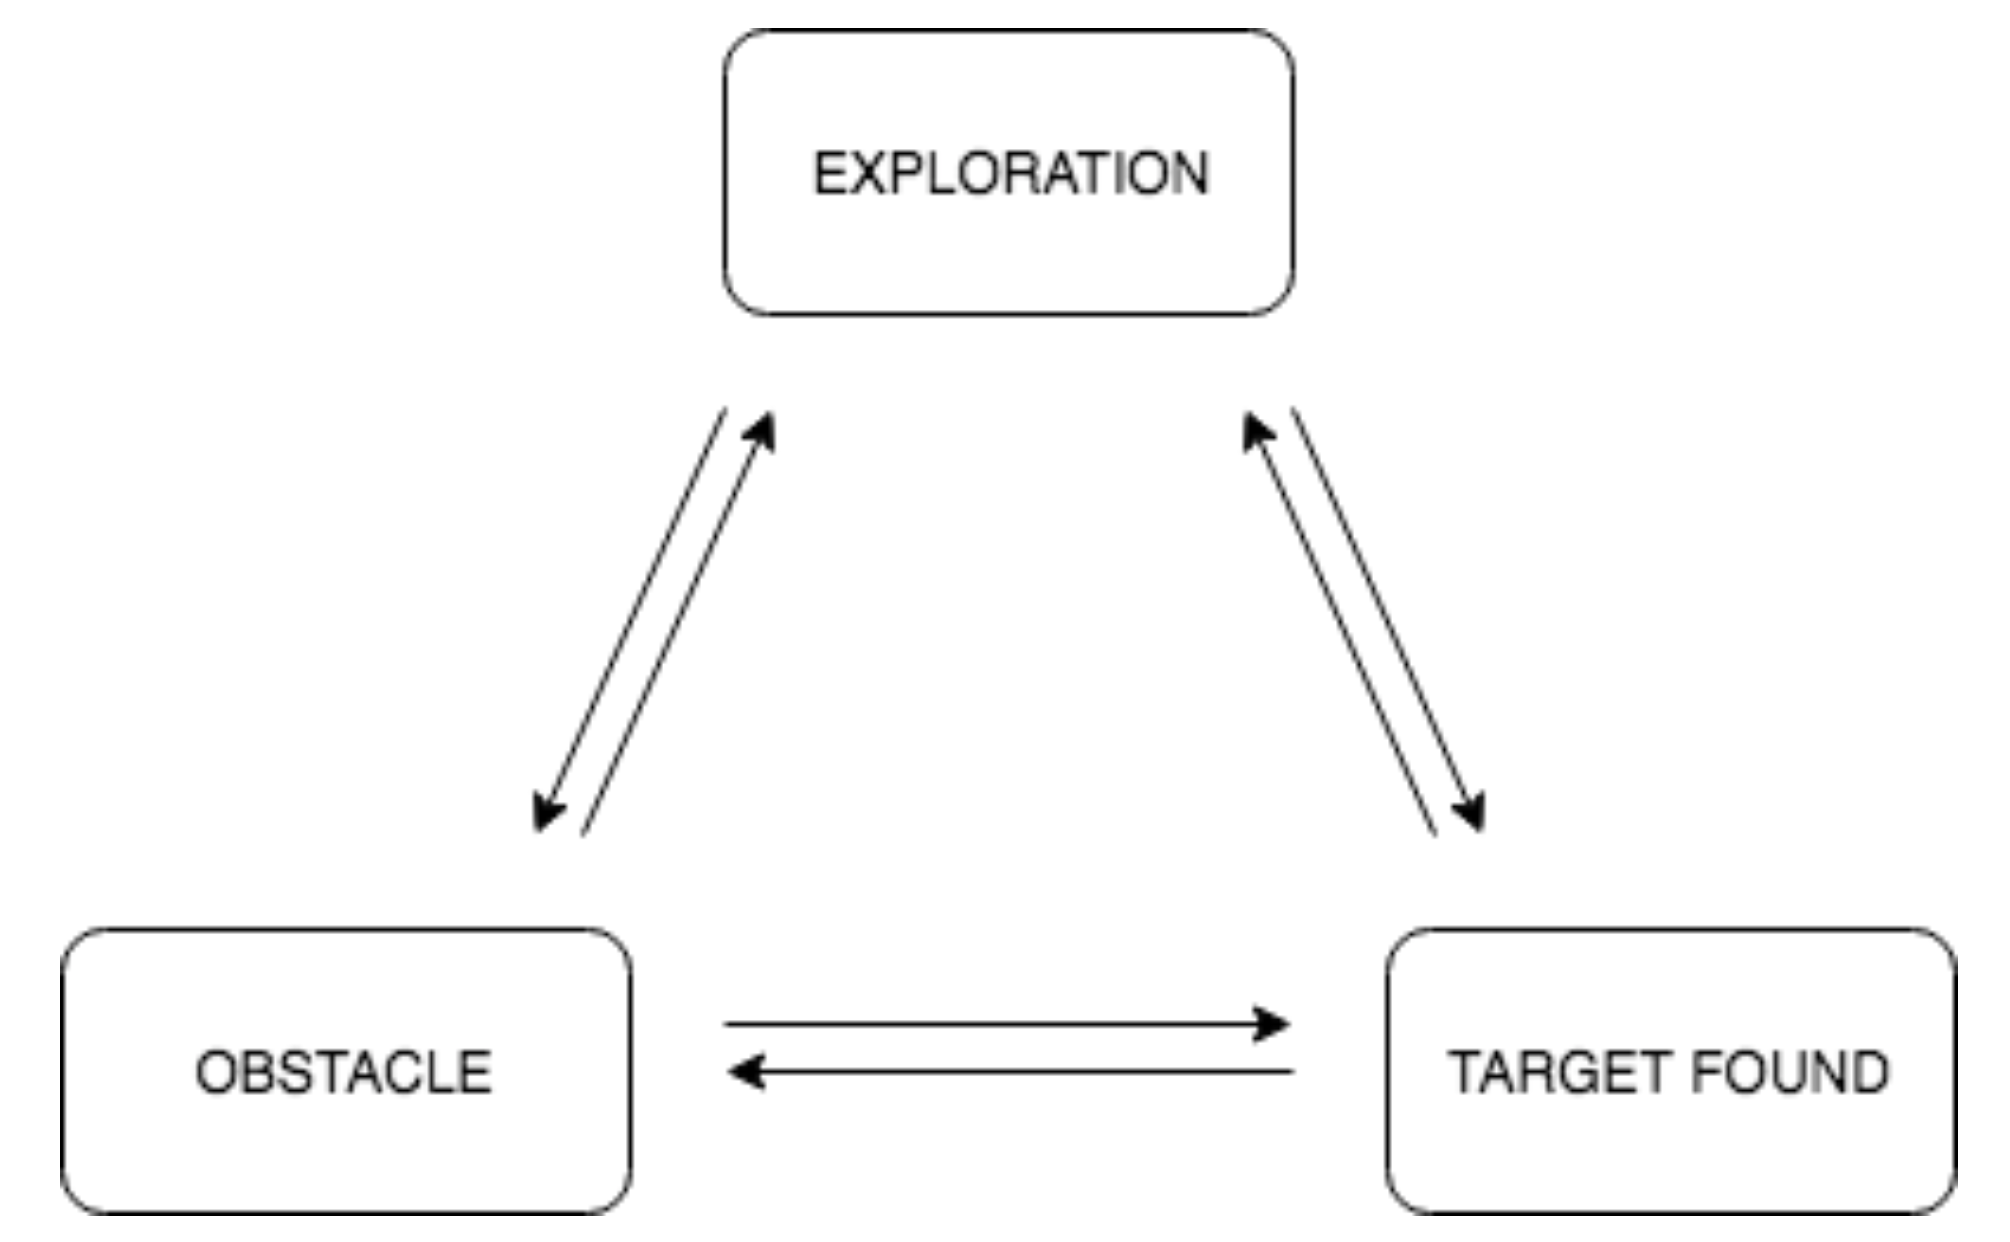
\includegraphics[width=\linewidth]{images/state}
\caption{State Machine}
\end{figure}
Thus, at any time the machine can be \textbf{only} in one of the three states: \emph{exploration}, \emph{obstacle} and \emph{target found}. 

\paragraph{Exploration} The robot starts to spin on itself with a fixed angular velocity to scan the surrounding until it finds the target or it detect an obstacle.
\paragraph{Target Found} When we find the object we are looking for, we start moving towards it by keeping the its bounding box in the camera's center. We used a Proportional Integral Derivative, PID, controller to select the correct angular velocity. Given the camera's image and the bounding box we define the error at time $t$ as:
\begin{equation}
e_t =  (l_b + \frac{w_b}{2}) - \frac{w_c}{2}
\end{equation}
Where, $w_c$ is the camera's image width, in our case 640, $l_b$ and $w_b$ are the left component and the width of target's bounding box respectively. To find $w_b$ we need to just subtract the the left and right component of the box. We are not taking the absolute value of the error since the sign is used to decide in which direction to turn. Before feeding  the error to the PID controller we normalise it between zero and one by dividing by $w_c$, otherwise we should have defined a very small proportional parameter for the PID. 

After we calculate the error for the current box, we feed it to a PID with a proportional parameter of $0.5$, and integral of $0$ and a derivative of $3$. However, even if we did not do any hyperparameter search, we notice that even with smaller values of the derivative component of the PID the robot works properly. 

The following figure shows the error for each frame given different position of the target class \emph{bottle}.
\begin{figure}[H]
\begin{center}
	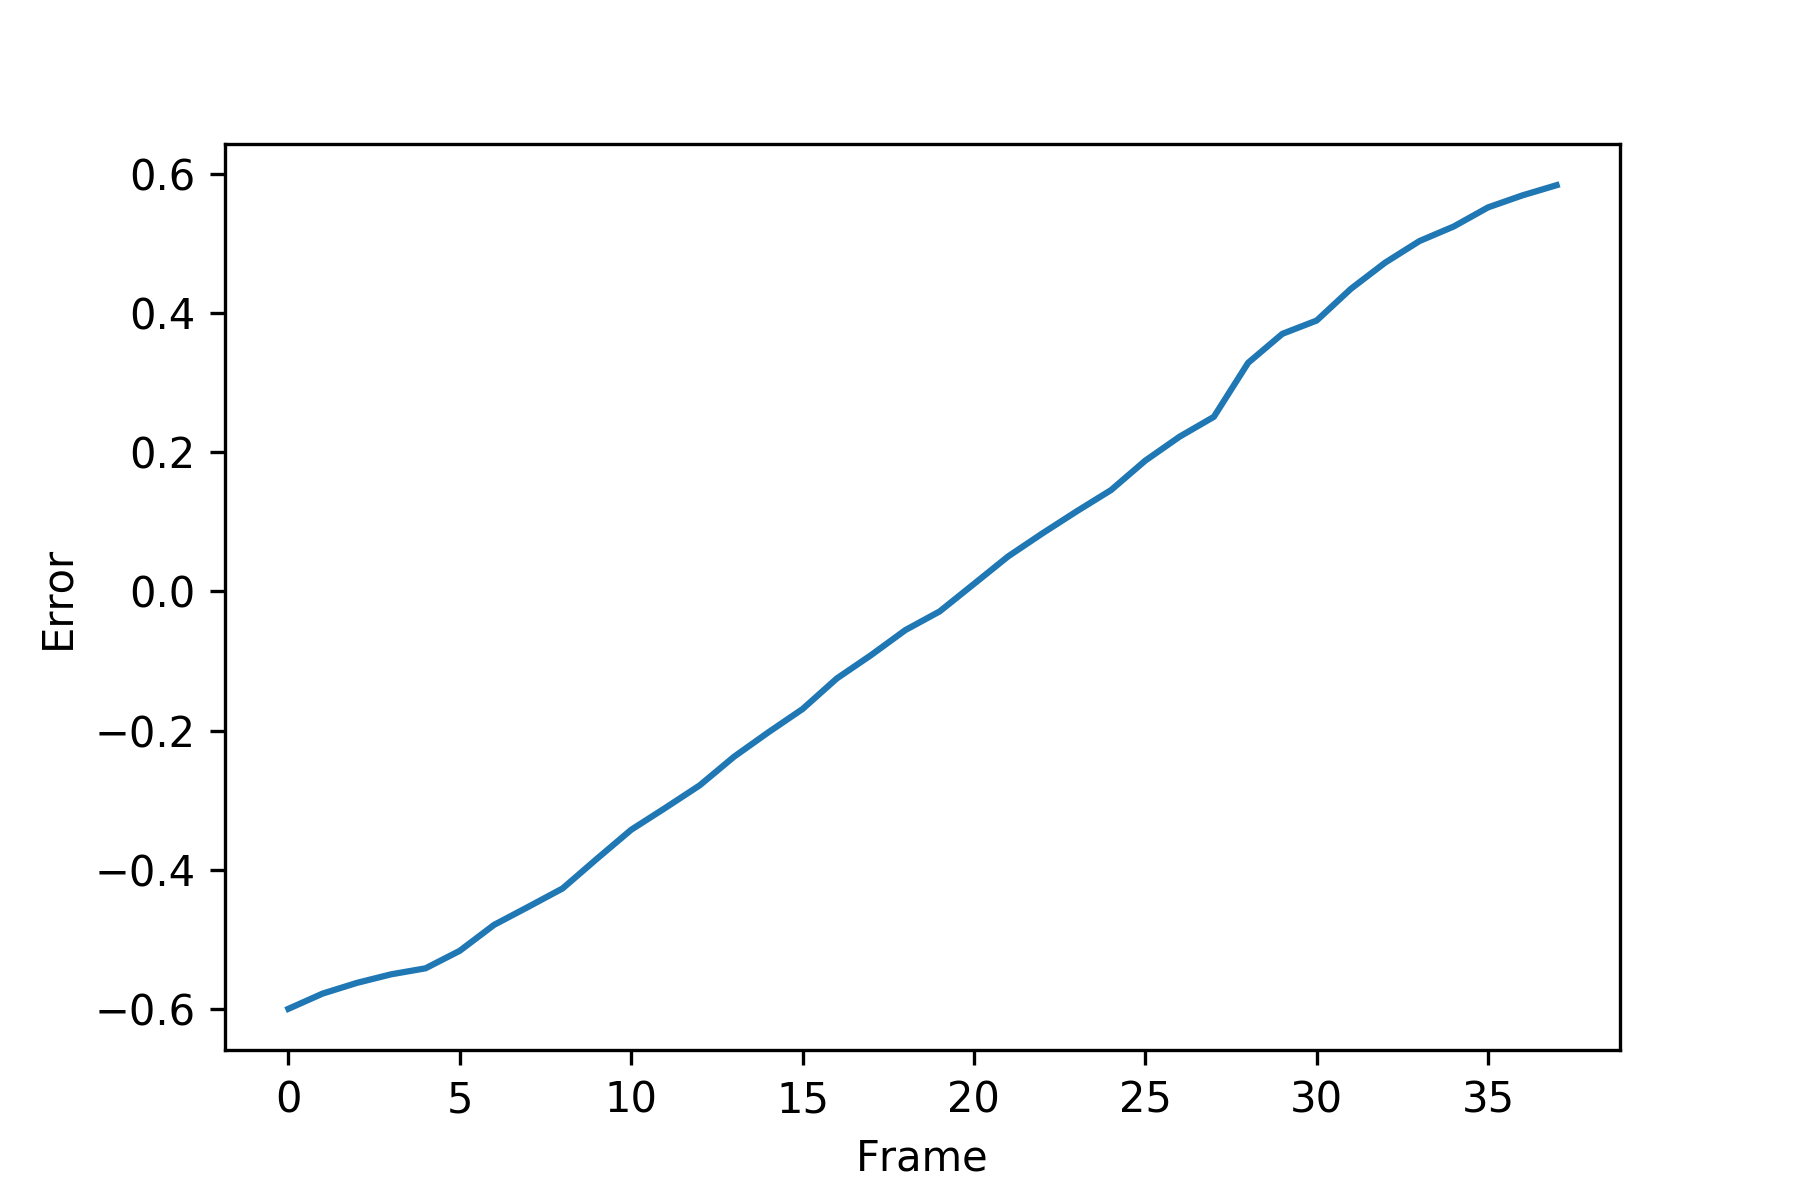
\includegraphics[width=\linewidth]{images/frame_error.png}
\end{center}	
\begin{center}
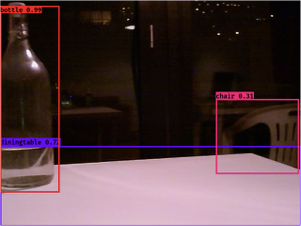
\includegraphics[width=0.25\linewidth]{images/bottle/1}	
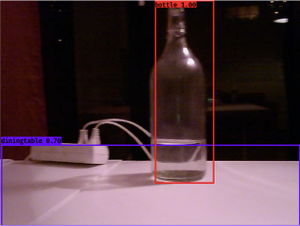
\includegraphics[width=0.25\linewidth]{images/bottle/2}	
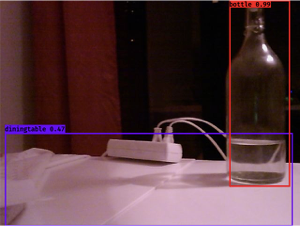
\includegraphics[width=0.25\linewidth]{images/bottle/3}		
\end{center}
\caption{Bounding Box Error}
\end{figure}
The error is bigger when the bottle is on the left on the right and it is zero when it is in the center of the image. We used it as angular velocity in order to keep the robot pointed to the target object. We move it forward with a fixed linear velocity of $0.1$. 

\paragraph{Obstacle} When the Thymio's proximity sensors of the Thymios, five in the front and two in the back, detect something it stops any activity and goes into the \emph{Obstacle} state. We implemented a simple yet effective PID controllers based algorithm to move the Thymio await from any object in from of it. 
We defined two PIDs, one for the linear velocity and one for the angular. The errors are $e_l$ for the linear PID and $e_a$ for the angular PID, defined as follow. We denote the front sensor set as $S_f$ and the rear sensor set as $S_r$, where each element in the set is a double representing the value from the sensor. In out case, $|S_f| = 5$ and $|S_r|=2$.
\begin{align}
	e_l &= \limits\sum_{i=0}^{|S_f|} S_f(i) - \limits\sum_{i = 0}^{|R_f|} R_f(i) \\
	e_a &= (\limits\sum_{i=0}^{\frac{|S_f|}{2}} S_f(i) - \limits\sum_{i = \frac{|S_f|}{2} }^{|S_f|} S_f(i)) - 
	(\limits\sum_{i=0}^{\frac{|R_f|}{2}} R_f(i) - \limits\sum_{i = \frac{|R_f|}{2} }^{|R_f|} R_f(i))
	\end{align}

Also, we turn on the five frontal Thymio's LED as user feedback.The number and position of the LEDs are based on the width of target's bounding box. For example, a big object on the left side will turn on two LEDs, while a smaller one only  one. The follow picture shows an example where the robot is looking for a \emph{cup}:
\begin{figure}[H]
\begin{center}
	
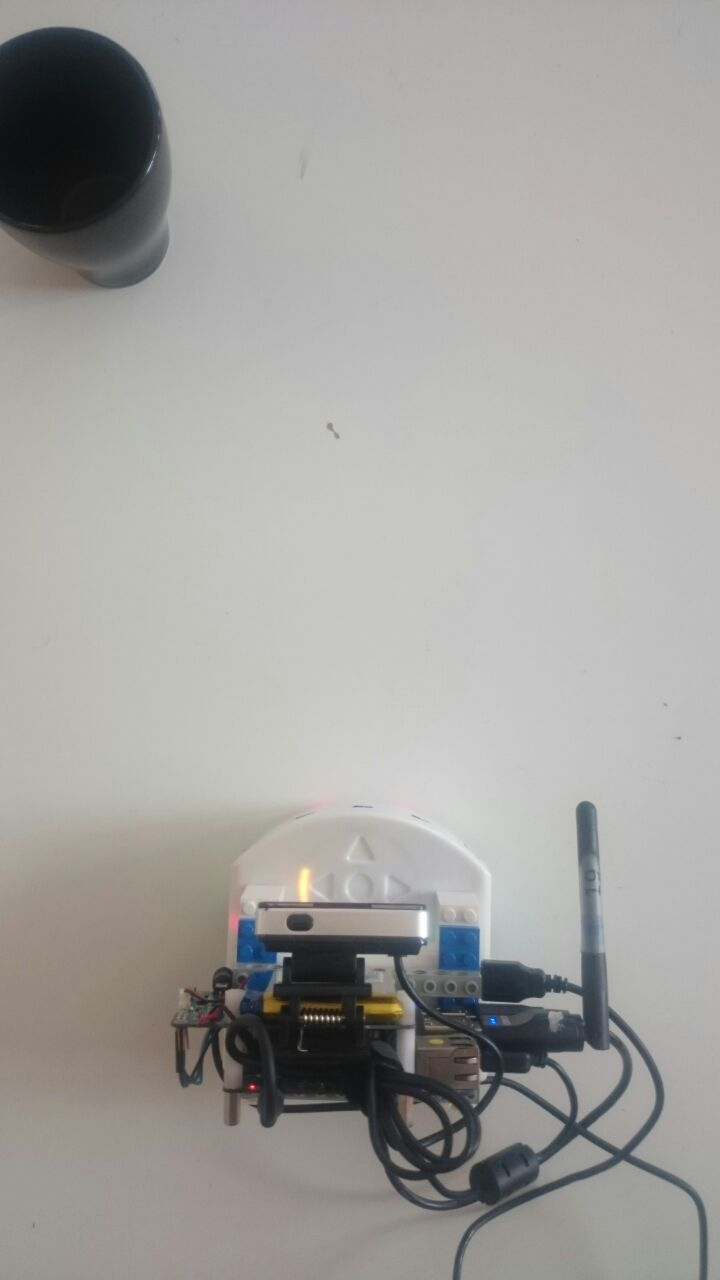
\includegraphics[width=0.25\linewidth]{images/leds/1}	
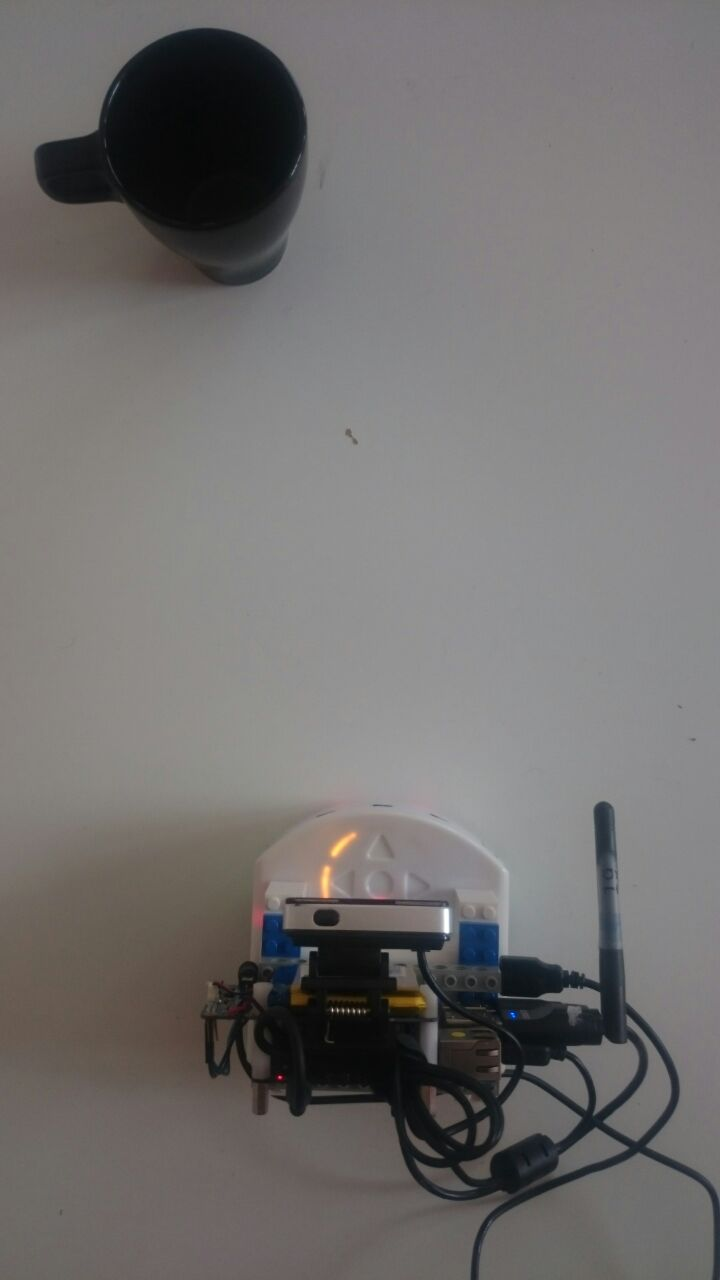
\includegraphics[width=0.25\linewidth]{images/leds/2}	
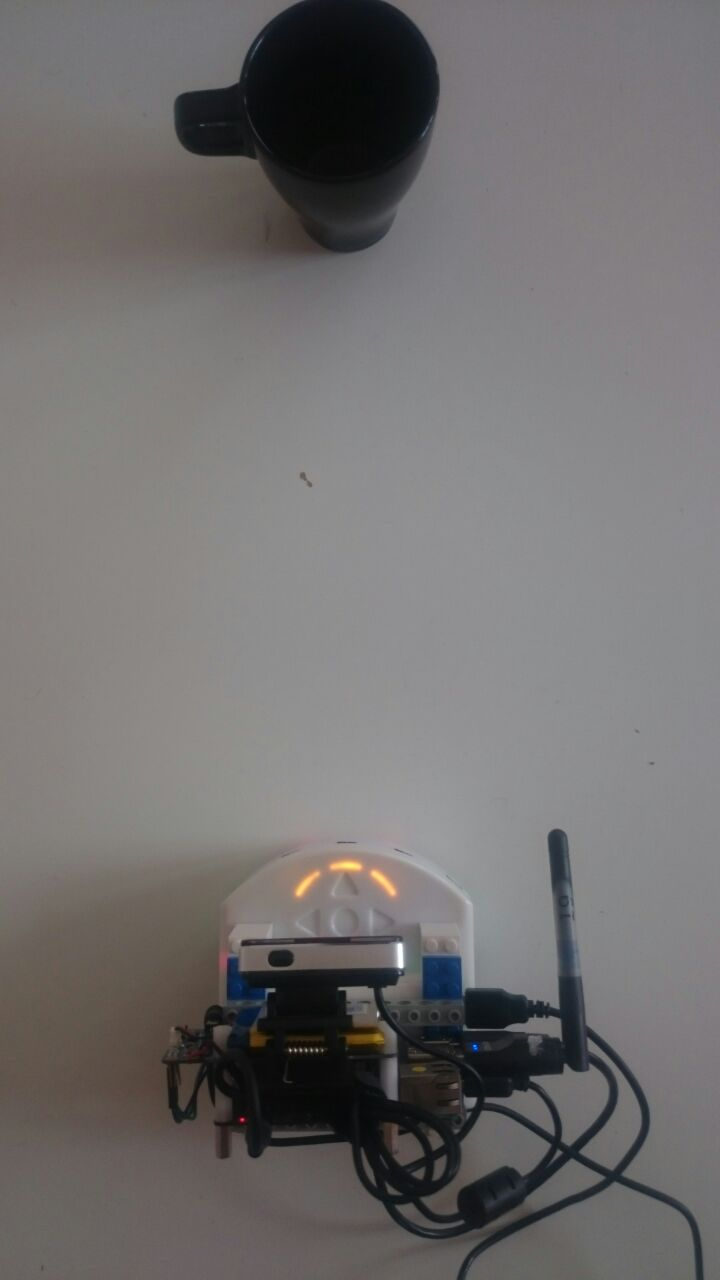
\includegraphics[width=0.25\linewidth]{images/leds/3}	
\end{center}
\begin{center}
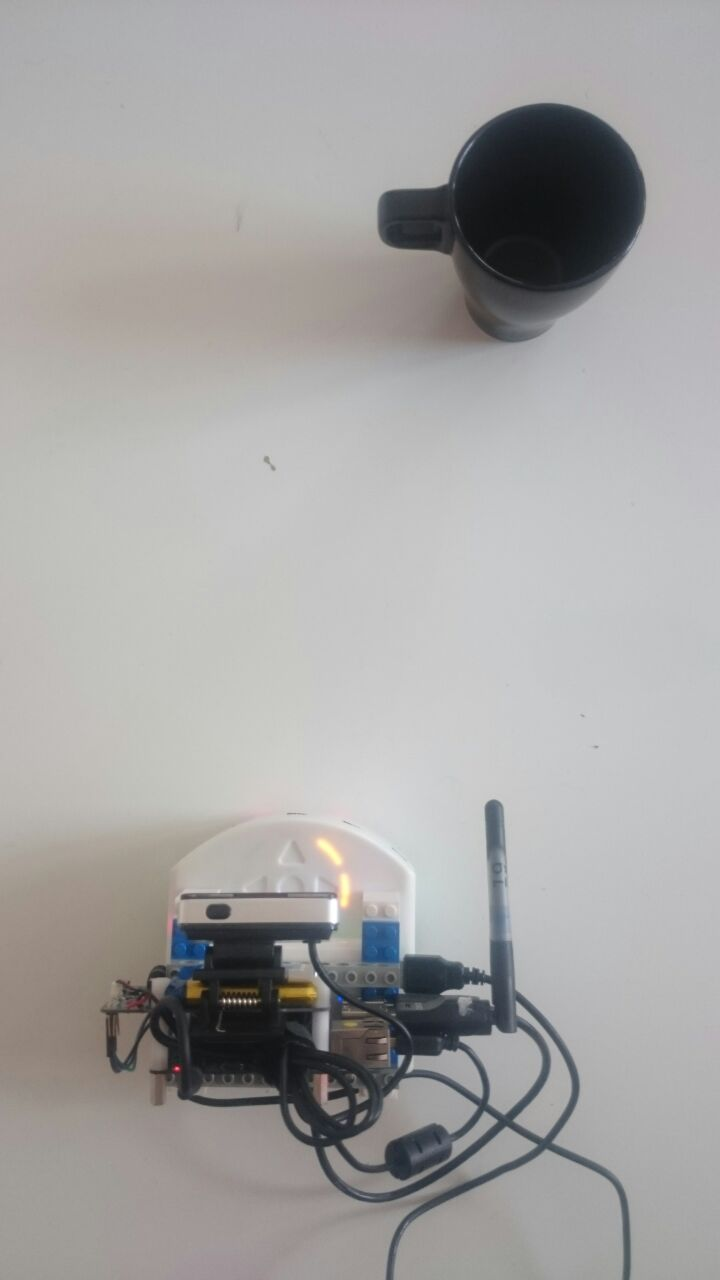
\includegraphics[width=0.25\linewidth]{images/leds/4}	
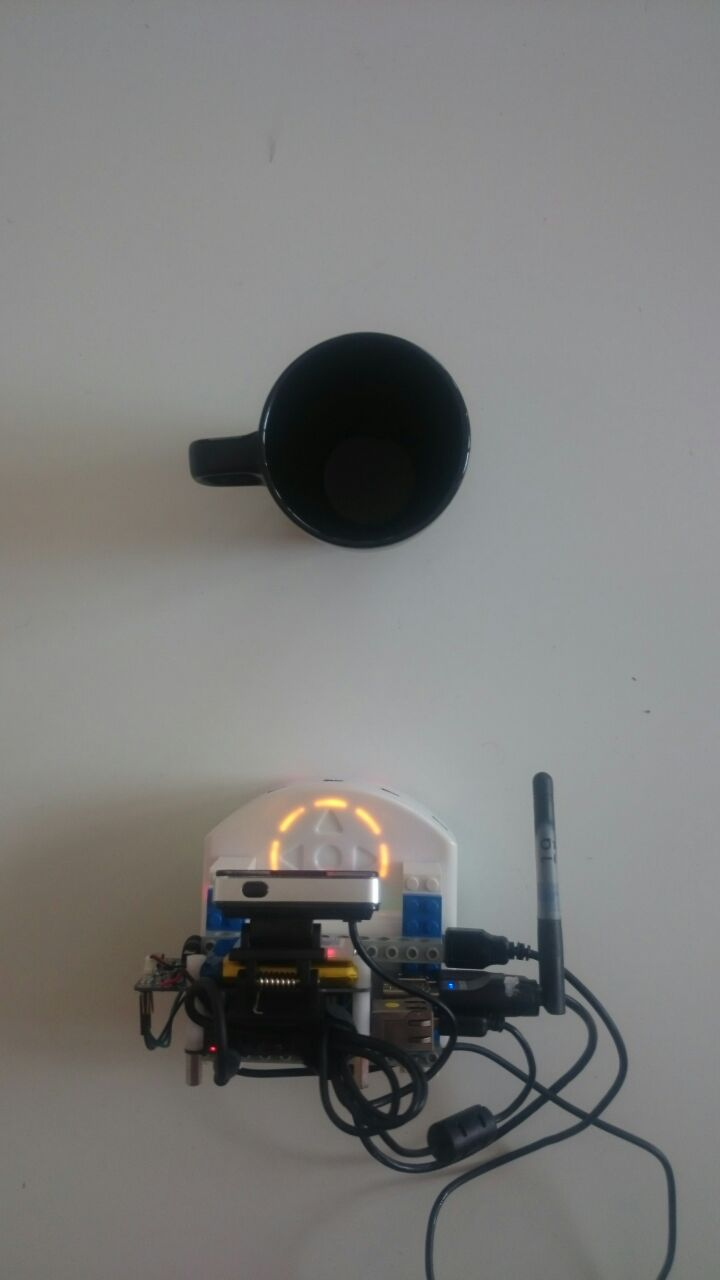
\includegraphics[width=0.25\linewidth]{images/leds/5}
\end{center}
\caption{On board LEDs}
\end{figure}

\section{Server}

\section{Results}

\section{Conclusion}
In this paper we presented a light and scalable architecture that uses a real-time Object Detection model to correctly find objects in the surrounding environment and to perform actions based on that. Since we only require a camera, our work can be used into similar robots running ROS with the correct hardware in order to extend their functionalities. Furthermore, since we used YOLO to perform the classification task, the model can be easily re-trained with other classes to expand the context domain. This symbiosis between Machine Learning and Robotic highlights the power of both areas by creating new interesting user cases and scenarios in which both disciplines can shine.

\printbibliography

%\begin{thebibliography}{99}
%%%%%% Our bibliography
%\bibitem{c1} Y. Redmon, S. Divvala, R. Girshick, and A. Farhadi, ÒYou Only Look Once: Unified, Real-Time Object Detection,Ó University of Washington, Allen Institute for AI, Facebook AI Research, May 2016, http://pjreddie.com/yolo/.
%\bibitem{c2} Y. Redmon, and A. Farhadi, ÒYOLOv3: An Incremental Improvement,Ó University of Washington, Apr 2018.
%
%\bibitem{c3} Guzzi, Jérôme and Giusti, Alessandro and Di Caro, Gianni A. and Gambardella, Luca M.,Mighty Thymio for Higher-Level Robotics Education, IDSIA, 2018.

%%%%%  Bibliography templates
%\bibitem{c1} G. O. Young, ÒSynthetic structure of industrial plastics (Book style with paper title and editor),Ó 	in Plastics, 2nd ed. vol. 3, J. Peters, Ed.  New York: McGraw-Hill, 1964, pp. 15Ð64.
%\bibitem{c2} W.-K. Chen, Linear Networks and Systems (Book style).	Belmont, CA: Wadsworth, 1993, pp. 123Ð135.
%\bibitem{c3} H. Poor, An Introduction to Signal Detection and Estimation.   New York: Springer-Verlag, 1985, ch. 4.
%\bibitem{c4} B. Smith, ÒAn approach to graphs of linear forms (Unpublished work style),Ó unpublished.
%\bibitem{c5} E. H. Miller, ÒA note on reflector arrays (Periodical styleÑAccepted for publication),Ó IEEE Trans. Antennas Propagat., to be publised.
%\bibitem{c6} J. Wang, ÒFundamentals of erbium-doped fiber amplifiers arrays (Periodical styleÑSubmitted for publication),Ó IEEE J. Quantum Electron., submitted for publication.
%\bibitem{c7} C. J. Kaufman, Rocky Mountain Research Lab., Boulder, CO, private communication, May 1995.
%\bibitem{c8} Y. Yorozu, M. Hirano, K. Oka, and Y. Tagawa, ÒElectron spectroscopy studies on magneto-optical media and plastic substrate interfaces(Translation Journals style),Ó IEEE Transl. J. Magn.Jpn., vol. 2, Aug. 1987, pp. 740Ð741 [Dig. 9th Annu. Conf. Magnetics Japan, 1982, p. 301].
%\bibitem{c9} M. Young, The Techincal Writers Handbook.  Mill Valley, CA: University Science, 1989.
%\bibitem{c10} J. U. Duncombe, ÒInfrared navigationÑPart I: An assessment of feasibility (Periodical style),Ó IEEE Trans. Electron Devices, vol. ED-11, pp. 34Ð39, Jan. 1959.
%\bibitem{c11} S. Chen, B. Mulgrew, and P. M. Grant, ÒA clustering technique for digital communications channel equalization using radial basis function networks,Ó IEEE Trans. Neural Networks, vol. 4, pp. 570Ð578, July 1993.
%\bibitem{c12} R. W. Lucky, ÒAutomatic equalization for digital communication,Ó Bell Syst. Tech. J., vol. 44, no. 4, pp. 547Ð588, Apr. 1965.
%\bibitem{c13} S. P. Bingulac, ÒOn the compatibility of adaptive controllers (Published Conference Proceedings style),Ó in Proc. 4th Annu. Allerton Conf. Circuits and Systems Theory, New York, 1994, pp. 8Ð16.
%\bibitem{c14} G. R. Faulhaber, ÒDesign of service systems with priority reservation,Ó in Conf. Rec. 1995 IEEE Int. Conf. Communications, pp. 3Ð8.
%\bibitem{c15} W. D. Doyle, ÒMagnetization reversal in films with biaxial anisotropy,Ó in 1987 Proc. INTERMAG Conf., pp. 2.2-1Ð2.2-6.
%\bibitem{c16} G. W. Juette and L. E. Zeffanella, ÒRadio noise currents n short sections on bundle conductors (Presented Conference Paper style),Ó presented at the IEEE Summer power Meeting, Dallas, TX, June 22Ð27, 1990, Paper 90 SM 690-0 PWRS.
%\bibitem{c17} J. G. Kreifeldt, ÒAn analysis of surface-detected EMG as an amplitude-modulated noise,Ó presented at the 1989 Int. Conf. Medicine and Biological Engineering, Chicago, IL.
%\bibitem{c18} J. Williams, ÒNarrow-band analyzer (Thesis or Dissertation style),Ó Ph.D. dissertation, Dept. Elect. Eng., Harvard Univ., Cambridge, MA, 1993. 
%\bibitem{c19} N. Kawasaki, ÒParametric study of thermal and chemical nonequilibrium nozzle flow,Ó M.S. thesis, Dept. Electron. Eng., Osaka Univ., Osaka, Japan, 1993.
%\bibitem{c20} J. P. Wilkinson, ÒNonlinear resonant circuit devices (Patent style),Ó U.S. Patent 3 624 12, July 16, 1990. 




\end{document}
